\documentclass{article}
\usepackage{../../Self_Style}

%setup hyperlink within pdf
\hypersetup{
    colorlinks=true,
    linkcolor=blue,
    filecolor=magenta,      
    urlcolor=cyan,
    pdftitle={Overleaf Example},
    pdfpagemode=FullScreen,
}

\title{Phys 20AL Lab Report Week 1: Pendulum}
\author{Zih-Yu Hsieh}
\date{\today}

\begin{document}
\maketitle

\tableofcontents

\hfil

\section{Introduction and Goal of the Experiment}
%explain what pendulums are, basic formulas, and the aim for the experiment (study relationships between length, mass, period of the pendulum)+ derive 
Under humans' observations, Pendulum is a physical system that obtains similar time period for each cycle when the amplitude of the cycles considered are small enough relative to the arm of the pendulum. Equivalently, one can also say this similarity occurs when the angle of the arm away from the bottom (the equilibrium point) is approximately $0$.

Under small angle approximation, the formula physicists derived for the pendulum's period is $\tau\approx 2\pi\sqrt{\frac{g}{l}}$ second (unit abbreviated as s), given that $l$ is the length of the arm of the pendulum (in units of meters m), and $g \approx 9.807$ m/s$^2$ (meters per second square) is the gravitational acceleration near Earth's surface.

The aim for this experiment includes:
\begin{itemize}
    \item Observe the (human observable) relationships between the mass $m$, the arm length $l$, and the period $\tau$ of a simple pendulum.
    \item Calculate how well the formula of period mentioned above approximates the actual period under fixed small angle.
    \item Use the experimental data to calculate gravitational acceleration $g$ near Earth's surface.
\end{itemize}

\pagebreak

\section{Experimental Setup}
The equipments for this experiment include: A stand, a protractor, a clip, a tape measure, a timer, a mass scale, a string with negligible mass, and multiple spherical weighted objects (each with different mass, depending on the lab equipment's availability).

The setup of the experiment goes as follow:
\begin{itemize}
    \item[1.] Fix the stand at the edge of the lab table, and fix the protractor horizontally on the top of the stand for measuring the pendulum arm's angle away from the equilibrium point.
    \item[2.] Tie / fix one end of the string to the clip, and clip it onto the stand. This is used for controlling the length of the pendulum's arm (or the length of the string that is hanged under the pivot).
    \item[3.] Put the other end of the string through a hole on the top of the stand, which serves as a pivot for the pendulum.
    \item[4.] Hang the spherical object(s) that serve as the mass of the pendulum at the end of the string that passes through the hole in 3.
\end{itemize}
\begin{figure}[h!]
    \centering
    \begin{subfigure}[t]{0.3\textwidth}
        \centering
        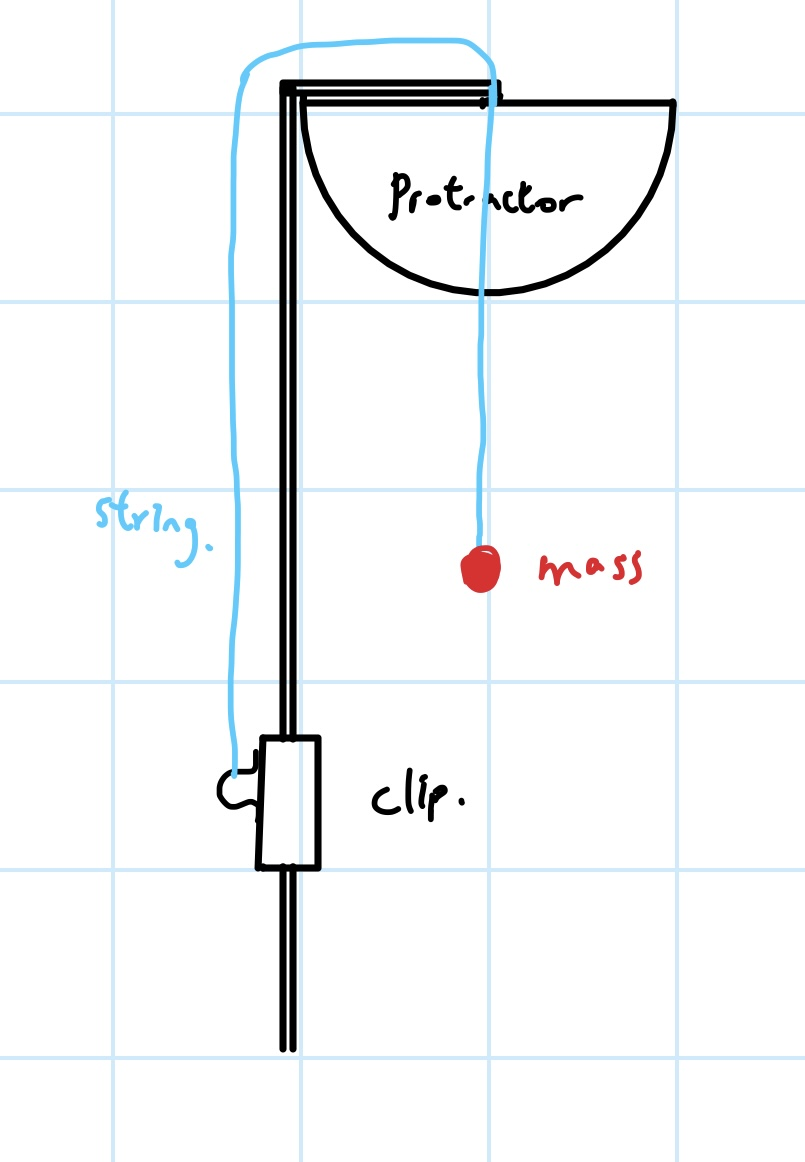
\includegraphics[width=\linewidth]{setup_sketch.png}
        \caption{Sketch of the Equipment Setup}
        \label{fig:sketch_setup}
    \end{subfigure}%
    \hfil 
    \begin{subfigure}[t]{0.2\textwidth}
        \centering
        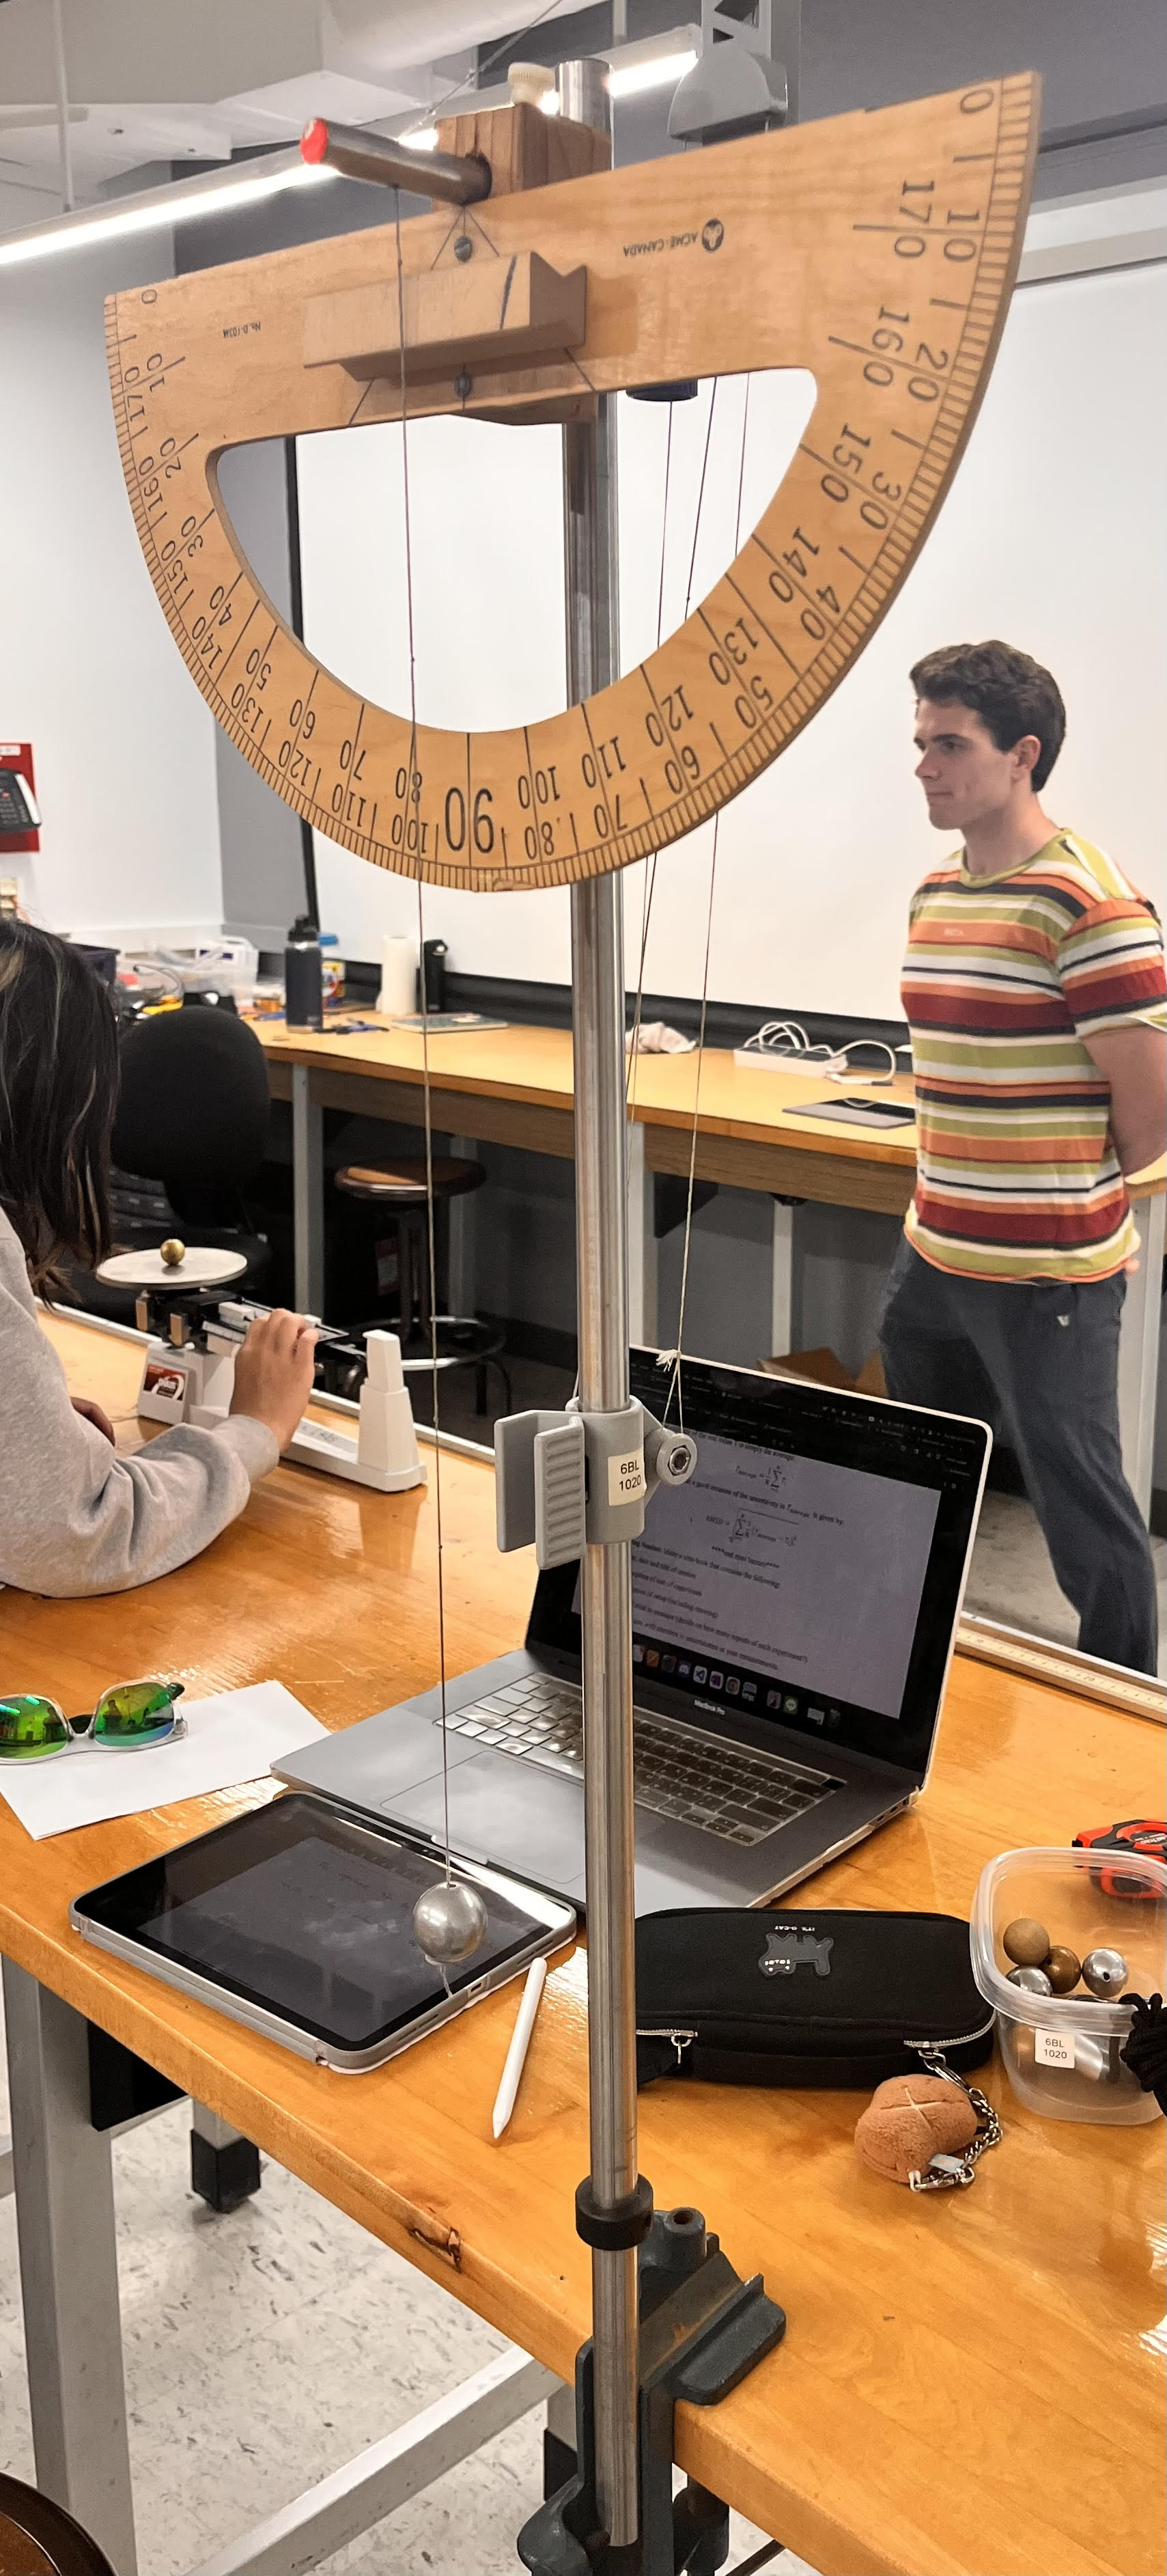
\includegraphics[width=\linewidth]{lab_setup.jpg}
        \caption{Photo of the Equipment Setup}
        \label{fig:physical_setup}
    \end{subfigure}
\end{figure}

\pagebreak

\section{Procedure and Methods of Measurement}
For each individual trial we'll record the length $l$ of the pendulum using tape measure, use the mass scale to measure the hanged mass $m$ on the pendulum, and use the timer to measure the period $\tau$ of the pendulum.

The independent variables include length $l$ and mass $m$ of the pendulum, which we'll test trials for each of the following combination:
\begin{itemize}
    \item The lengths of the pendulum used are $0.3$m, $0.4$m, $0.5$m, and $0.6m$. 
    \item The masses of the pendulum used are $5.5$g, $20$g, $66$g, and $71.5$g (based on the provided objects in the lab). 
\end{itemize}
The dependent variable of the experiment is the period $\tau$ of the pendulum, while the rest of the factors are considered as controlled variables.

For the experiment, we'll follow the procedure below:
\begin{itemize}
    \item[1.] First, choose a mass for the pendulum, hang it onto the string, then fix a length for the pendulum by adjusting the position of the clip.
    \item[2.] Raise the pendulum till it is $10^\circ$ away from equilibrium (check it with the protractor) and release.
    \item[3.] Wait for the pendulum to complete $5$ cycles, then record the period for the $6^\textmd{th}$ cycle using the timer.
    \item[4.] Repeat Step 2 and 3 five times with fixed mass and length.
    \item[5.] Change the length of the pendulum to a different one await to be experimented with, and repeat Step 2 to 4 for each length.
    \item[6.] Change the mass of the pendulum to a different one await to be experimented with, and repeat Step 2 to 5 for each desired mass.
\end{itemize}
The purpose is to observe the effect of the pendulum length on the period of the pendulum under fixed mass and other conditions, then compare the variation of the overall effects when masses are changed.

\pagebreak

\section{Experimental Data and Tables}
\begin{table}[ht!]
    \centering

    % First row
    \begin{subtable}[t]{0.4\textwidth}
        \centering
        \caption{Mass: 5.5g}
        \begin{tabular}{c||c|c|c|c|c}
            \toprule
            \diagbox[width=3cm,height=1cm]{Length (m)}{Trial} & 1 & 2 & 3 & 4 & 5 \\
            \midrule
            0.3 & 1.08 & 1.04 & 1.13 & 1.15 & 1.06 \\
            \hline
            0.4 & 1.26 & 1.33 & 1.23 & 1.24 & 1.18 \\
            \hline
            0.5 & 1.41 & 1.48 & 1.38 & 1.43 & 1.39 \\
            \hline
            0.6 & 1.49 & 1.53 & 1.49 & 1.58 & 1.48 \\
            \bottomrule
        \end{tabular}
        \label{tab:mass_5.5g}
    \end{subtable}
    \hfill
    \begin{subtable}[t]{0.4\textwidth}
        \centering
        \caption{Mass: 20g}
        \begin{tabular}{c||c|c|c|c|c}
            \toprule
            \diagbox[width=3cm,height=1cm]{Length (m)}{Trial} & 1 & 2 & 3 & 4 & 5 \\
            \midrule
            0.3 & 1.09 & 1.03 & 1.09 & 1.09 & 1.13 \\
            \hline
            0.4 & 1.06 & 1.29 & 1.29 & 1.19 & 1.24 \\
            \hline
            0.5 & 1.34 & 1.43 & 1.44 & 1.46 & 1.43 \\
            \hline
            0.6 & 1.59 & 1.51 & 1.58 & 1.51 & 1.53 \\
            \bottomrule
        \end{tabular}
        \label{tab:mass_20g}
    \end{subtable}

    \vspace{1em}

    % Second row
    \begin{subtable}[t]{0.4\textwidth}
        \centering
        \caption{Mass: 66g}
        \begin{tabular}{c||c|c|c|c|c}
            \toprule
            \diagbox[width=3cm,height=1cm]{Length (m)}{Trial} & 1 & 2 & 3 & 4 & 5 \\
            \midrule
            0.3 & 1.01 & 1.08 & 1.11 & 1.04 & 1.09 \\
            \hline
            0.4 & 1.19 & 1.26 & 1.29 & 1.24 & 1.28 \\
            \hline
            0.5 & 1.34 & 1.43 & 1.44 & 1.46 & 1.43 \\
            \hline
            0.6 & 1.48 & 1.58 & 1.54 & 1.48 & 1.63 \\
            \bottomrule
        \end{tabular}
        \label{tab:mass_66g}
    \end{subtable}
    \hfill
    \begin{subtable}[t]{0.4\textwidth}
        \centering
        \caption{Mass: 71.5g}
        \begin{tabular}{c||c|c|c|c|c}
            \toprule
            \diagbox[width=3cm,height=1cm]{Length (m)}{Trial} & 1 & 2 & 3 & 4 & 5 \\
            \midrule
            0.3 & 1.11 & 1.03 & 1.06 & 1.08 & 1.07 \\
            \hline
            0.4 & 1.23 & 1.23 & 1.34 & 1.21 & 1.23 \\
            \hline
            0.5 & 1.39 & 1.39 & 1.41 & 1.33 & 1.43 \\
            \hline
            0.6 & 1.54 & 1.54 & 1.53 & 1.51 & 1.58 \\
            \bottomrule
        \end{tabular}
        \label{tab:mass_71.5g}
    \end{subtable}

    \caption{Measured oscillation periods (unit: second s) for different masses and string lengths}
    \label{tab:period}
\end{table}

\begin{table}[ht!]
    \centering
    %first row
    \begin{subtable}[t]{0.4\textwidth}
        \centering
        \caption{Mass: 5.5g}
        \begin{tabular}{c||c||c}
            \toprule
            Length (m) & Average Period (s) & SD \\
            \midrule
            0.3 & 1.092 & 0.047\\
            \hline
            0.4 & 1.248 & 0.054\\
            \hline
            0.5 & 1.418 & 0.040\\
            \hline
            0.6 & 1.514 & 0.042\\
            \bottomrule
        \end{tabular}
        \label{tab:mass_5.5g_1}
    \end{subtable}
    \hfill
    \begin{subtable}[t]{0.4\textwidth}
        \centering
        \caption{Mass: 20g}
        \begin{tabular}{c||c||c}
            \toprule
            Length (m) & Average Period (s) & SD \\
            \midrule
            0.3 & 1.086 & 0.036\\
            \hline
            0.4 & 1.214 & 0.096\\
            \hline
            0.5 & 1.42 & 0.046\\
            \hline
            0.6 & 1.544 & 0.038\\
            \bottomrule
        \end{tabular}
        \label{tab:mass_5.5g_1}
    \end{subtable}
    \vspace{1em}

    %bottom
    \begin{subtable}[t]{0.4\textwidth}
        \centering
        \caption{Mass: 66g}
        \begin{tabular}{c||c||c}
            \toprule
            Length (m) & Average Period (s) & SD \\
            \midrule
            0.3 & 1.066 & 0.040\\
            \hline
            0.4 & 1.252 & 0.040\\
            \hline
            0.5 & 1.42 & 0.046\\
            \hline
            0.6 & 1.542 & 0.065\\
            \bottomrule
        \end{tabular}
        \label{tab:mass_5.5g_1}
    \end{subtable}
    \hfill
    \begin{subtable}[t]{0.4\textwidth}
        \centering
        \caption{Mass: 71.5g}
        \begin{tabular}{c||c||c}
            \toprule
            Length (m) & Average Period (s) & SD \\
            \midrule
            0.3 & 1.07 & 0.029\\
            \hline
            0.4 & 1.248 & 0.052\\
            \hline
            0.5 & 1.39 & 0.037\\
            \hline
            0.6 & 1.54 & 0.025\\
            \bottomrule
        \end{tabular}
        \label{tab:mass_5.5g_1}
    \end{subtable}
    \caption{The Average Period, and Standard Deviation of the previous Data}
    \label{tab:data}
\end{table}

\begin{figure}[ht!]
    \centering
    %top row
    \begin{subfigure}{0.49\textwidth}
        \centering
        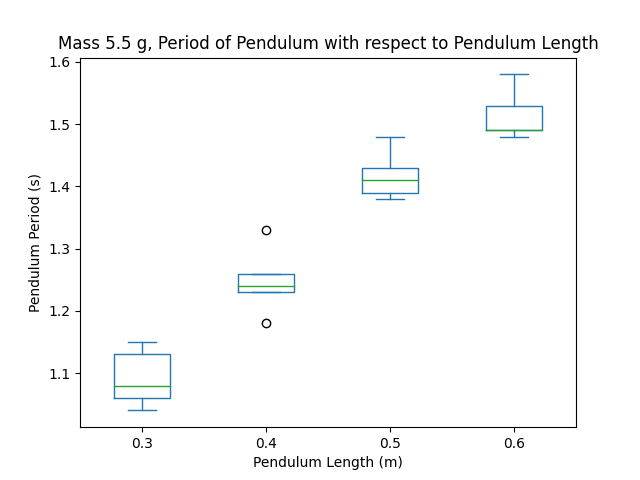
\includegraphics[width=\linewidth]{mass1.png}
        \label{fig:graph_m1}
    \end{subfigure}
    \hfil
    \begin{subfigure}{0.49\textwidth}
        \centering
        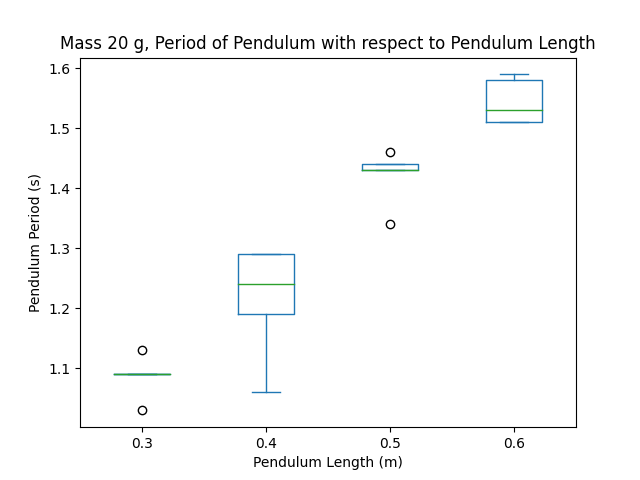
\includegraphics[width=\linewidth]{mass2.png}
        \label{fig:graph_m2}
    \end{subfigure}

    \vspace{1em}

    %bottom row
    \begin{subfigure}{0.49\textwidth}
        \centering
        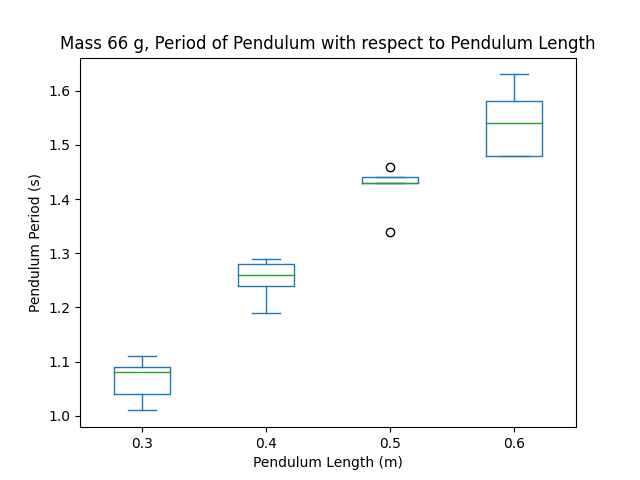
\includegraphics[width=\linewidth]{mass3.png}
        \label{fig:graph_m3}
    \end{subfigure}
    \hfil
    \begin{subfigure}{0.49\textwidth}
        \centering
        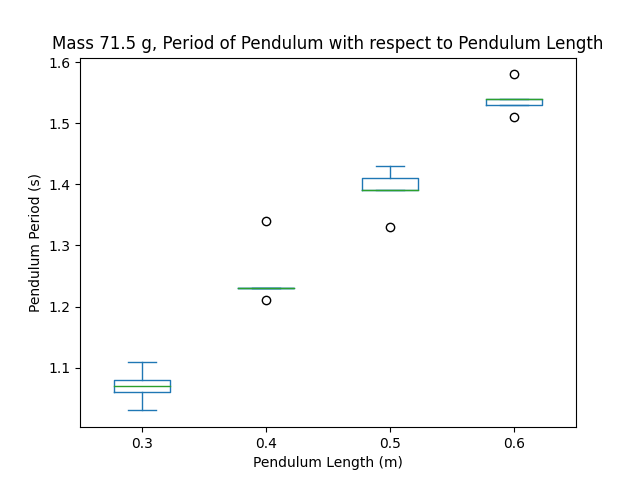
\includegraphics[width=\linewidth]{mass4.png}
        \label{fig:graph_m4}
    \end{subfigure}
    \caption{The Diagram of Experimental Data with Distribution}
    \label{fig:graphs}
\end{figure}

\pagebreak

\hfil

\pagebreak

\section{Data Analysis}
From Table \ref{tab:data} and Figure \ref{fig:graphs}, one can see for each pair of mass and length, the standard deviation of the pendulum's period (for the five trials experimented) are all in between $0.025$ second to $0.096$ second. The standard deviations for each mass and length pair is relatively small compared to the standard time length of $1$ second, hence the collected data for each mass and length pair is highly concentrated. So, it has high validity of using the average for comparison.

\hfil

Which, taken the average periods given in Table \ref{tab:data} for each masses, they form the following table:

\begin{table}[ht!]
    \centering
        \begin{tabular}{c||c|c|c|c||c||c}
            \toprule
            \diagbox[width=3cm,height=1cm]{Length (m)}{Mass (g)} & 5.5 & 20 & 66 & 71.5 & Average & SD \\
            \midrule
            0.3 & 1.092 & 1.086 & 1.066 & 1.07 & 1.079 & 0.012\\
            \hline
            0.4 & 1.248 & 1.214 & 1.252 & 1.248 & 1.241 & 0.018\\
            \hline
            0.5 & 1.418 & 1.42 & 1.42 & 1.39 & 1.412 & 0.015\\
            \hline
            0.6 & 1.514 & 1.544 & 1.542 & 1.54 & 1.535 & 0.014\\
            \bottomrule
        \end{tabular}
        \caption{Table of Average Periods (unit: s), their Average by Length, and Standard Deviation}
        \label{tab:average}
\end{table}

From the above table one can observe that given a fixed length, the standard deviation of the average periods (when varying mass) is controlled in between $0.012$ to $0.018$ s, which is also relatively small compared to the standard time period $1$ s. Hence, when fixing the length, the average time period is still highly concentrated when varying the mass, which indicates there is a high confidence that change of mass doesn't affect the pendulum's period, when given the setup of small amplitude.

Due to the small value of standard deviation, it also indicates that the average of these average time periods (when fixing length) are valid representatives of the pendulum's time period of the fixed length.

\hfil

Now, given length $l = 0.3,0.4,0.5,0.6$ m, with $g=9.807$ m/s$^2$, the period of the pendulum predicted by the formula is given by $\tau = 2\pi \sqrt{\frac{l}{g}} \approx 1.147, 1.269, 1.419, 1.554$ s respectively. If using the ``average'' of the average periods derived in Table \ref{tab:average} as the representatives, they provide the following table:
\begin{table}[ht!]
    \centering
    \begin{tabular}{c||c|c|c|c}
        \toprule
        Length (m) & 0.3 & 0.4 & 0.5 & 0.6\\
        \hline
        Average Period (s) & 1.079 & 1.248 & 1.39 & 1.535\\
        \hline
        Predicted Period (s) & 1.147 & 1.269 & 1.419 & 1.554\\
        \hline
        \hline
        Percent Error (\%) & 6.302 & 1.683 & 2.086 & 1.238\\
        \bottomrule
    \end{tabular}
    \caption{Comparison of Average Period with Formula Prediction}
    \label{tab:compare}
\end{table}

Which, the above table demonstrates the collected data's average has a percent error between $1.238$ to $6.302$ \%, showing the experimental data is close to the predicted period. This verifies the period formula $\tau = 2\pi\sqrt{\frac{l}{g}}$ for given length $l$, is a good approximation of the actual period presented in the experiment.

\pagebreak

\section{Error Analysis}
Some possible human mistakes observed when doing the experiment includes:
\begin{itemize}
    \item Human eyes' measurement error, which possibly occurs when measuring the length of the pendulum, and the angle of the pendulum before releasing.
    \item Human's reaction time, which possibly occurs when using the timer to record the period.
\end{itemize}
For the possible error in the experiment includes:
\begin{itemize}
    \item Friction and Air Resistance, which the variation of these factors across the experiment cause the amplitude of the pendulum at the $5^\textmd{th}$ cycle to be varying, which has a potential of affecting the results.
    \item Pendulum itself is not a perfect simple pendulum, since regardless of the material, the string used for pendulum still has some mass, while the mass hanged at the bottom is also not a point mass. These slight deviation from the ideal scenario could also cause potential error to arise.
\end{itemize}

\hfil

\section{Calculation of Gravitational Acceleration $g$}
Recall that the formula $\tau = 2\pi\sqrt{\frac{l}{g}}$ predicts the pendulum's period $\tau$ (unit: s) when given the pendulum's length $l$ (unit: m). By doing some algebraic manipulation, the gravitational constant $g = l\left(\frac{2\pi}{\tau}\right)^2$.

Apply this formula to all experimental data, it produces the following table (on the next page):
\begin{table}[ht!]
    \centering
    % First row
    \begin{subtable}[t]{0.4\textwidth}
        \centering
        \caption{Mass: 5.5g}
        \begin{tabular}{c||c|c|c|c|c}
            \toprule
            \diagbox[width=3cm,height=1cm]{Length (m)}{Trial} & 1 & 2 & 3 & 4 & 5 \\
            \midrule
            0.3 & 10.154 & 10.950 & 9.275 & 8.955 & 10.541 \\ 
            \hline
            0.4 & 9.947 & 8.927 & 10.438& 10.270 & 11.341\\
            \hline
            0.5 & 9.929 & 9.012 & 10.365 & 9.653 & 10.216 \\
            \hline
            0.6 & 10.669 & 10.119 & 10.669 & 9.488 & 10.814 \\
            \bottomrule
        \end{tabular}
        \label{tab:mass_5.5g}
    \end{subtable}

    \vspace{1em}

    \begin{subtable}[t]{0.4\textwidth}
        \centering
        \caption{Mass: 20g}
        \begin{tabular}{c||c|c|c|c|c}
            \toprule
            \diagbox[width=3cm,height=1cm]{Length (m)}{Trial} & 1 & 2 & 3 & 4 & 5 \\
            \midrule
            0.3 & 9.968 & 11.164 & 9.968 & 9.968 & 9.275 \\
            \hline
            0.4 & 14.054 & 9.489 & 9.489 & 11.151 & 10.270\\
            \hline
            0.5 & 10.993 & 9.653 & 9.518 & 9.260 & 9.653 \\
            \hline
            0.6 & 9.369 & 10.389 & 9.488 & 10.389 & 10.119\\
            \bottomrule
        \end{tabular}
        \label{tab:mass_20g}
    \end{subtable}

    \vspace{1em}

    % Second row
    \begin{subtable}[t]{0.4\textwidth}
        \centering
        \caption{Mass: 66g}
        \begin{tabular}{c||c|c|c|c|c}
            \toprule
            \diagbox[width=3cm,height=1cm]{Length (m)}{Trial} & 1 & 2 & 3 & 4 & 5 \\
            \midrule
            0.3 & 11.610 & 10.154 & 9.612 & 10.950 & 9.968\\
            \hline
            0.4 & 11.151 & 9.947 & 9.489 & 10.270 & 9.638\\
            \hline
            0.5 & 10.993 & 9.653 & 9.519 & 9.260 & 9.653\\
            \hline
            0.6 & 10.814 & 9.488 & 9.988 & 10.814 & 8.915\\
            \bottomrule
        \end{tabular}
        \label{tab:mass_66g}
    \end{subtable}

    \vspace{1em}

    \begin{subtable}[t]{0.4\textwidth}
        \centering
        \caption{Mass: 71.5g}
        \begin{tabular}{c||c|c|c|c|c}
            \toprule
            \diagbox[width=3cm,height=1cm]{Length (m)}{Trial} & 1 & 2 & 3 & 4 & 5 \\
            \midrule
            0.3 & 9.612 & 11.164 & 10.541 & 10.154 & 10.345\\
            \hline
            0.4 & 10.438 & 10.438 & 8.794 & 10.786 & 10.438\\
            \hline
            0.5 & 10.216 & 10.216 & 9.929 & 11.159 & 9.653\\
            \hline
            0.6 & 9.988 & 9.988 & 10.119 & 10.389 & 9.488\\
            \bottomrule
        \end{tabular}
        \label{tab:mass_71.5g}
    \end{subtable}

    \caption{Calculated Gravitational Acceleration (unit: m/s$^2$) for each Trial}
    \label{tab:g}
\end{table}

Which, the calculated average is $g_\textmd{ave}\approx 10.139$ m/s$^2$, while the standard deviation $\sigma \approx 0.777$ m/s$^2$. 

The derived gravitational acceleration compared to the current agreed value $g=9.807$ m/s$^2$, has a Percent Error of about $3.27$\%.

\pagebreak

\hfil

\pagebreak

\section{Conclusion}
In this lab, the experimental data suggests that under small angle, there is a high confidence that the time period of the pendulum is independent from the mass, and dependent on the length of the pendulum. And, by comparison the period formula $\tau = 2\pi\sqrt{\frac{l}{g}}$ provides the period values close to what is demonstrated in current experiment, showing it is a valid approximation in this experiment specifically.

Finally, the calculated gravitational acceleration in this experiment is $g_\textmd{ave}\approx 10.139$ m/s$^2$, with the current agreed value $g=9.807$ m/s$^2$, the Percent Error is about $3.27$\%, which is considered close to the agreed value.

\hfil

Besides the human measurement mistakes (including human's reaction time and uncertainty when measuring using raw eyes), some possible experimental error that may affect the results include friction and air resistance (which potentially lower the amplitude of the pendulum when measuring), and also the fact that the system is not perfectly a simple pendulum.

\end{document}